\section{Einleitung}
	Samplesort ist ein vergleichsbasierter, In-Place, Sortieralgorithmus, der 1970 zuerst vorgestellt wurde. \autocite{frazer-1970}
	Dabei ist Samplesort eine Generalisierung des Quicksort und für große Datenmengen ausgelegt, bei denen andere Algorithmen, wie z.B. der klassische Quicksort oder Insertion Sort, durch eine bereits vorhandene Teilsortierung, nicht performant sind.
	Auch ist Samplesort besonders effizient darin, viele Prozessorkerne möglichst effizient auszunutzen.
	Aus diesem Grund findet er vor allem in hoch Skalierten Systemen, mit vielen Daten, Anwendung.\\
	Deshalb wird er, auch wenn er über 50 Jahre alt ist, heute noch verwendet.
	Mit der Zeit gab es allerdings viele Optimierungen und Abweichungen vom Original.
	Im Folgenden ist die Zugrundeliegende Sortierproblematik für die verschiedenen Anwendungsfälle differenziert dargestellt, sowie wie Samplesort funktioniert, wann seine Vorteile die anderer Algorithmen übertreffen und welche Variationen wann am besten sind.
	
	\subsection{Sortierproblematik}
		Schon seit Anbeginn der theoretischen Informatik sind Sortieralgorithmen weit diskutiert.
		Heute sind viele verschiedene Algorithmen bekannt, um verschiedene Anreihungen von Daten, auf die unterschiedlichsten Arten zu sortieren.
		Eine Eigenschaft hat sich dabei besonders herausgestellt und so wird im Folgenden nur Bezug auf vergleichsbasierte Sortieralgorithmen genommen.\footnote{Nicht vergleichsbasierte Sortieralgorithmen sind mit klassischer Hardware nicht umsetzbar und in der Regel Algorithmen für Hardwarekomponenten. So ist für Integer auch eine Laufzeit von $O(n)$ möglich. \autocite{abdel-hafeez-2017}}
		Diese müssen ein Minimum von $\log_2{n!}$ Vergleichen durchführen, um jedes Element eindeutig einordnen zu können, und haben damit eine minimale Laufzeitkomplexität von $\Omega(\log_2{n!})$.\footnote{$O(f(x))$ ist die maximal begrenzte, $\Omega(f(x))$ die minimal begrenzte und $\Theta(f(x))$ die übereinstimmende maximal und minimal begrenzte Laufzeit. $O$, $\Omega$ und $\Theta$ beschreiben dabei einen konstanten Faktor. \autocite[4]{sedgewick-1996}}
	
		\paragraph{Aspekte eines Sortieralgorithmus}
			Die Auswahl des richtigen Algorithmus kann dabei, abhängig vom Verwendungsfall, von verschiedenen Faktoren abhängig sein.\\
			Die klassischen Beispiele sind \textbf{Laufzeit} und benötigter zusätzlicher \textbf{Speicher}.
			Wenn komplexe Strukturen, wie Dateien, die einen hohen Aufwand zum Laden benötigen, sortiert werden sollen, dann ist auch wichtig, wie viele Vergleiche der Algorithmus durchführt, da diese in dem Fall sehr zeitaufwändig sind.
			Dem gegenüber stehen Systeme, die sehr lange für das Tauschen der Position (Swap) in der zu sortierenden Datenstruktur benötigen.
			Dauert das Schreiben länger, als das Lesen der Daten, wird die Anzahl der Vergleiche in Relation weniger relevant.\\
			Besonders wichtig für uns ist das Verhindern der Entartung so wie die möglichkeit zur parallelisierung.
			Aber auch, ob der Algorithmus \textbf{stabil} ist, also die ursprüngliche Reihenfolge gleichwertiger Elemente gewährleistet ist, können eine Rolle spielen.\\
			

	\subsection{Was ist Samplesort?}
		Bei all diesen Kriterien schneidet Quicksort im Schnitt am besten ab, stößt aber auch schnell an seine Grenzen. 
		Sind die Daten in umgekehrter sortierter Reihenfolge vorhanden, so steigert sich seine Laufzeit von durchschnittlich $O(n\log{n})$ auf $\Omega(n^2)$ (Entartung).\\
		\begin{figure}
			\caption{Laufzeitkomplexitäten \autocite{unknown-author-2021}}
			\centering
			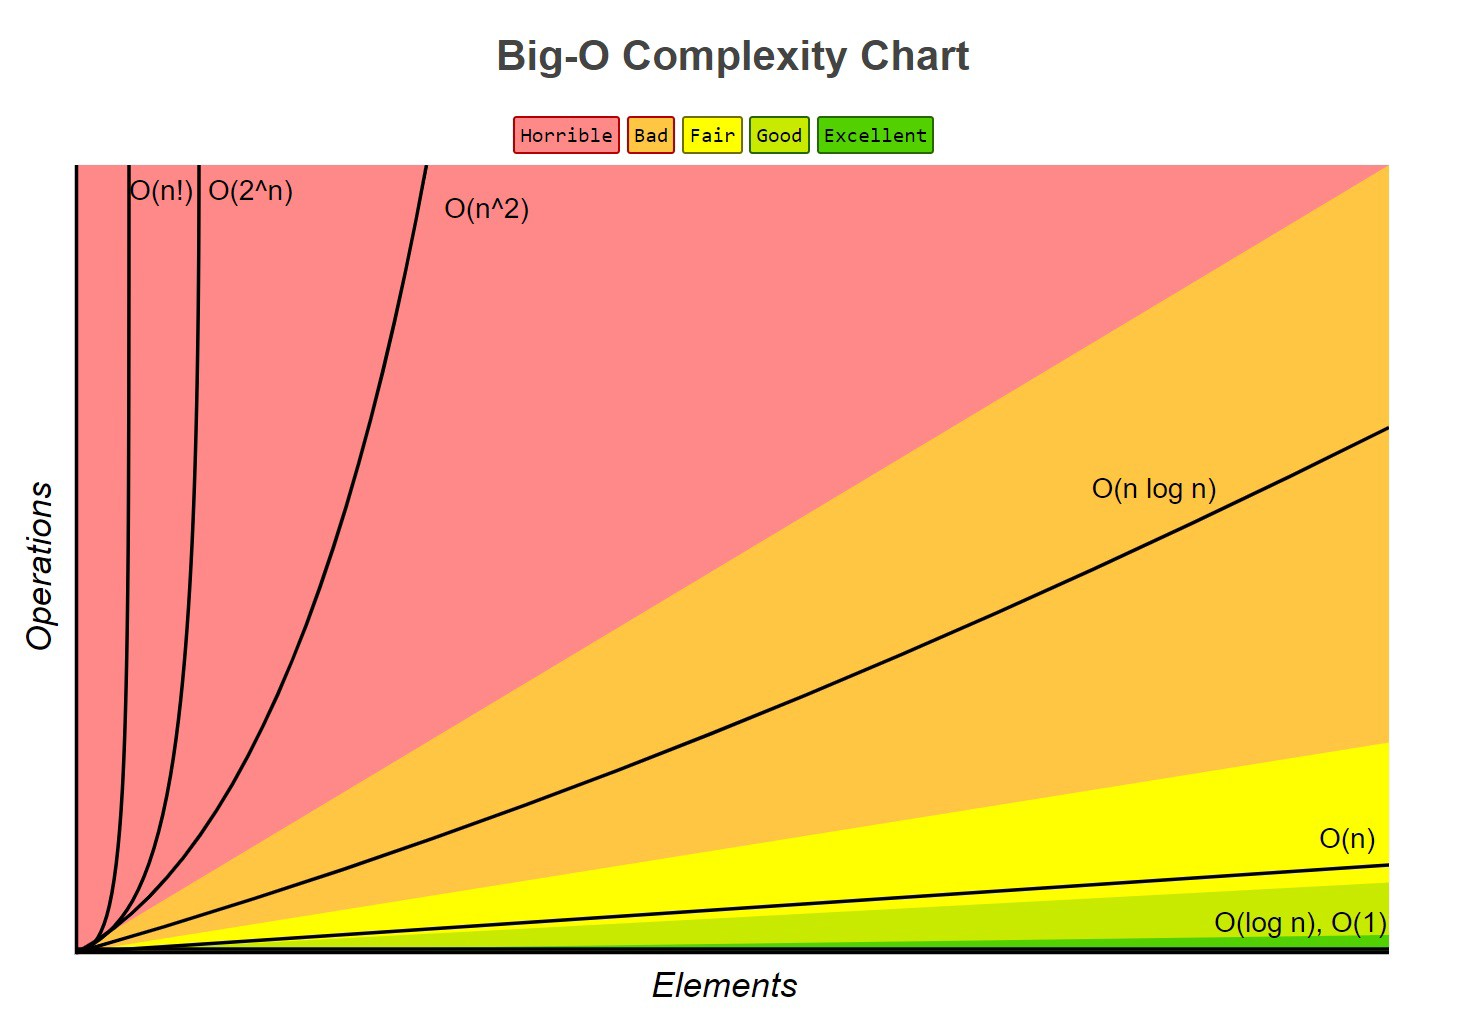
\includegraphics[width=\paperwidth-2in]{bigo.jpeg}
		\end{figure}
		Dieser Fall erscheint zunächst selten, doch wenn, zum Beispiel, neue Nutzerdaten jeden Tag um Mitternacht neu in eine strukturierte Datenbank übernommen werden sollen, ist dies häufig der Fall.\\
		Heapsort kann hier, mit einer Laufzeit von $\Theta(n\log{n})$ Abhilfe schaffen, ist aber im Schnitt langsamer als Quicksort.\\
		Samplesort ist eine Generalisierung von Quicksort:\\
		Während Quicksort ein Pivot Element hat\footnote{Hier ein Link für eine anschauliche Erklärung: \hyperlink{https://www.youtube.com/watch?v=0SkOjNaO1XY}{https://www.youtube.com/watch?v=0SkOjNaO1XY}}, hat Samplesort $p$ Pivot Elemente, auch Splitter genannt, wobei diese zufällig ausgewählt werden.
		Dadurch benötigt Samplesort im Schnitt 15\% weniger Vergleiche als Quicksort. \autocite{frazer-1970}
		Außerdem ist Samplesort für Systeme mit mehreren Prozessorkernen ausgelegt.
		So wird $p$ meistens als die Anzahl von Kernen - 1 definiert und durch die zufällige Auswahl der Splitter hat jeder Kern eine annähernd identische Last und der Algorithmus kann den vollen Prozessor nutzen, um schneller fertig zu werden.\\
